%%%%%%%%%%%%%%%%%%%%%%%%%%%%%%%%%%%%%%%%%%%%%%
%% Template Thesis DGH UW v3.0
%%
%% Vincent Labatut 04/2015
%% Grégoire Lurton 07/2015
%%
%% v1   - 10/2014 : forme de rapport très différente
%% v2   - 02/2015 : modèle complètement refait
%% v2.1 - 03/2015 : définition de la page de titre
%% v2.2 - 03/2015 : correction de quelques bugs
%% v2.3 - 04/2015 : page de titre complétée (date, adresse postale, long titre)
%% v3.0 - 07/2015 : adaptation de la page de titre pour UW DGH
%% v3.1 - 07/2015 : inclusion de packages pour equations et test pour compilation knitr
%%%%%%%%%%%%%%%%%%%%%%%%%%%%%%%%%%%%%%%%%%%%%%
%\documentclass[a4paper,11pt,draft,twoside]{article}
\documentclass[a4paper,11pt,twoside]{article}

%%%%%%%%%%%%%%%%%%%%%%%%%%%%%%%%%%%%%%%%%%%%%%%%%%%
%% Loading Packages
%%%%%%%%%%%%%%%%%%%%%%%%%%%%%%%%%%%%%%%%%%%%%%%%%%%
\usepackage[english]{babel}
\usepackage[utf8]{inputenc}
\usepackage[T1]{fontenc}
\usepackage{mathpazo}
\usepackage{euler}
\usepackage[top=2.5cm, bottom=2.5cm, left=2.5cm, right=2.5cm]{geometry}
\usepackage{setspace}
\usepackage[french]{varioref}
\usepackage{lastpage}
\usepackage{fancyhdr}
\usepackage[table]{xcolor}
\usepackage{lmodern}
\usepackage{amsmath,amsthm,amscd,amssymb}
\PassOptionsToPackage{hyphens}{url}\usepackage{hyperref}

\usepackage{tikz}
\usetikzlibrary{decorations.pathreplacing , chains , intersections}
\usetikzlibrary{calc}

\usepackage{relsize}
\usepackage{pgfgantt}
\usepackage{pgfcalendar}

%%%%%%%%%%%%%%
\tikzset{
>=stealth',
    fontscale/.style = {font=\relsize{#1}} ,
    punktchain/.style={
            rectangle,
    rounded corners,
    draw=black, very thick,
    text width=10em,
    minimum height=3em,
    text centered,
    on chain},
  line/.style={draw, thick, <-},
  element/.style={
    tape,
    top color=white,
    bottom color=blue!50!black!60!,
    minimum width=8em,
    draw=blue!40!black!90, very thick,
    text width=10em,
    minimum height=3.5em,
    text centered,
    on chain},
  every join/.style={->, thick,shorten >=1pt},
  decoration={brace},
  tuborg/.style={decorate},
  tubnode/.style={midway, right=2pt},
}


%%%%%%%%%%%%%%%


\usepackage{natbib}


%%%%%%%%%%%%%%%%%%%%%%%%%%%%%%%%%%%%%%%%%%%%%%%%%%%
%% Paper's Information -- TO TWEAK
%%%%%%%%%%%%%%%%%%%%%%%%%%%%%%%%%%%%%%%%%%%%%%%%%%%
%TITLE
\newcommand{\reporttitle}{Local Health Metrics}

%AUTHORS
\newcommand{\reportauthors}{Grégoire Lurton}

%PROGRAM
\newcommand{\program}{PhD in Global Health}

%TRACK
\newcommand{\track}{Metrics Track}

%%%%%%%%%%%%%%%%%%%%%%%%%%%%%%%%%%%%%%%%%%%%%%%%%%%
%% Formatting stuff
%%%%%%%%%%%%%%%%%%%%%%%%%%%%%%%%%%%%%%%%%%%%%%%%%%%
\setlength{\headheight}{13.6pt} % due to a warning
\newcommand{\HRule}{\rule{\linewidth}{0.5mm}}
% Espace entre les paragraphes

% Headers and Footers
\pagestyle{fancy}
\fancyhf{}

\renewcommand{\headrulewidth}{0.4pt}
\renewcommand{\footrulewidth}{0.4pt}

\cfoot{\thepage}
\fancyhead[L]{\small\reporttitle}
\fancyhead[R]{\small\rightmark}

%%%% Define custom colors
\definecolor{grisclair}{rgb}{0.7,0.7,0.7}
\definecolor{grisfonce}{rgb}{0.5,0.5,0.5}
\definecolor{green}{RGB}{22,122,48}
\definecolor{red}{RGB}{163,45,29}
\definecolor{blue}{RGB}{20,86,101}
\definecolor{orange}{RGB}{163,96,29}
\definecolor{yellow}{rgb}{0.984375, 0.7265625, 0}


\newcommand{\sectionbreak}{\clearpage}


%%% PDF Metadatas
\hypersetup{
    pdftitle={\reporttitle},
    pdfauthor={\reportauthors},
    pdfsubject={\reporttitle},
    bookmarksnumbered=true,bookmarksopen=true,
	unicode=true,colorlinks=true,linktoc=all,
	linkcolor=blue,citecolor=blue,filecolor=blue,urlcolor=blue,
	pdfstartview=FitH
}

%%% Font  - Get sans serif
\renewcommand{\familydefault}{\sfdefault}
%\fontfamily{garamond}



\DeclareUnicodeCharacter{00A0}{~}



% Get Bulleted Lists Working
%\renewcommand{\FrenchLabelItem}{\textbullet}

%%%%%%%%%%%%%%%%%%%%%%%%%%%%%%%%%%%%%%%%%%%%%%%%%%
%%% WATERMARK
%\usepackage{draftwatermark}
%\SetWatermarkText{DRAFT}
%\SetWatermarkScale{5}

% Load the package with the acronym option
\usepackage[acronym,nomain]{glossaries}

% Generate the glossary
\makeglossaries

\begin{document}
%%%%%%%%%%%%%%%%%%%%%%%%%%%%%%%%%%%%%%%%%%%%%%%%%%%
%% Title Page
%%%%%%%%%%%%%%%%%%%%%%%%%%%%%%%%%%%%%%%%%%%%%%%%%%%
\phantomsection
\begin{titlepage}
	\begin{tikzpicture}[remember picture,overlay]
		\node at (current page.south west)
		{
			\begin{tikzpicture}[remember picture,overlay]
				\pgftext[x=0cm,y=25.37cm,bottom,left]{
\includegraphics[width=21cm, draft = false]{images/dgh_banner.png}};
				\pgftext[x=1.1cm,y=24cm,bottom,left]{\fontsize{20}{20}{\textbf{\program}}};
				\pgftext[x=1.1cm,y=23.2cm,bottom,left]{\fontsize{18}{18}{\textbf{\textcolor{grisfonce}\track}}};
				\pgftext[x=10.5cm,y=16.5cm,bottom,center]{\fontsize{30}{30}{\textbf{Local Practice or Global Norm ?}}};%\reporttitle
				\pgftext[x=10.5cm,y=15.2cm,bottom,center]{\fontsize{30}{30}{\textbf{Exploring the border between}}};
                \pgftext[x=10.5cm,y=13.9cm,bottom,center]{\fontsize{30}{30}{\textbf{local and global Health Metrics}}};
				\pgftext[x=10.5cm,y=13.0cm,bottom,center]{\scalebox{0.77}[1]{\fontsize{20}{20}{\fontfamily{phv}\selectfont{}\textcolor{grisfonce}{\reportauthors}}}};
				%\pgftext[x=5.5cm,y=13.1cm,bottom,left]{\scalebox{0.6}[1]{\fontsize{18}{18}{\fontfamily{phv}\selectfont{}\textbf{\today}}}};
				\pgftext[x=1.1cm,y=1.8cm,bottom,left]{
\includegraphics[width=6cm , draft = false]{images/ihme_logo.png}};
				%\pgftext[x=9.1cm,y=1.8cm,bottom,left]{
\includegraphics[width=6cm, draft = false]{images/itech_logo.png}};
				%\pgftext[x=17.1cm,y=1.8cm,bottom,left]{
\includegraphics[width=3cm, draft = false]{images/bluesquare_logo.png}};
				\fill[fill=grisclair] (21cm,1cm) rectangle(0cm,0cm);
			\end{tikzpicture}
		};
	\end{tikzpicture}

\end{titlepage}

%% Get the page after title empty
\pagenumbering{gobble}% Remove page numbers (and reset to 1)
\newpage\null\thispagestyle{empty}\newpage


%%%%%%%%%%%%%%%%%%%%%%%%%%%%%%%%%%%%%%%%%%%%%%%%%%%%%%%%%%%%%%%%%%
%%%%    	FRONT MATTER
%%%%%%%%%%%%%%%%%%%%%%%%%%%%%%%%%%%%%%%%%%%%%%%%%%%%%%%%%%%%%%%%%%
\thispagestyle{plain}
\pagenumbering{roman}
\setcounter{page}{1}


\newacronym{cqi}{CQI}{Continuous Quality Improvement}
\newacronym{emr}{EMR}{Electronic Medical Record}
\newacronym{his}{HIS}{Health Information System}
\newacronym{hmis}{HMIS}{Health Management Information System}
\newacronym{rhis}{RHIS}{Routine Health Information System}
\newacronym{rdqa}{RDQA}{Routine Data Quality Assessment}
\newacronym{who}{WHO}{World Health Organization}

\paragraph{Abstract}

This proposal defines a project for a doctoral research into data processing and analysis methods adapted to Health Information Systems in developing countries. My research explores the relationship between local and global levels of analysis in Global Health Metrics.

I concentrate on three important dimensions of this relationship. First, I define an approach to local indicator definition. Using Electronic Medical Records data from HIV care in different countries, I show how the most common metric used for patients retention in HIV care is impacted by data quality and local characteristics, and I explore robust alternatives to this metric. Second, using widely available data from Niger, I  implement a data-hybridization strategy to produce an actionable map of Niger population. Finally, I develop an analytical framework to understand the relationship between health metrics and the political and social systems in which they are used.

This project will contribute to research in the Global Health Metrics field in different ways. It will contribute to the research, mainly from the Information and Communication Technologies for Development community, on flexible standards for data collection. It will offer a framework for the analysis and use of real-world data in low-resource settings. Finally, it will contribute to the Science and Technology Studies field by offering a framework the analysis of how quantitative methods in health systems are affected by the structures in which they are used, and how they can in return impact these structures.

% Table des matières
\cleardoublepage
% Dans le cas du recto verso, ajoute une page blanche si besoin
\phantomsection
\tableofcontents
\addcontentsline{toc}{section}{Table of Content}
\newpage
\addcontentsline{toc}{section}{\listfigurename}
\listoffigures
\newpage

%\addcontentsline{toc}{section}{\listtablename}
%\listoftables
%\newpage
\addcontentsline{toc}{section}{Acronyms}
\printglossaries
\thispagestyle{fancy}

% Justification moins stricte : des mots ne dépasseront pas des paragraphes
\sloppy

%%%%%%%%%%%%%%%%%%%%%%%%%%%%%%%%%%%%%%%%%%%%%%%%%%%
%%%% 	MAIN MATTER
%%%%%%%%%%%%%%%%%%%%%%%%%%%%%%%%%%%%%%%%%%%%%%%%%%%

%% Set page numbering right
\cleardoublepage
\pagenumbering{arabic}
\setcounter{page}{1}


\section{Introduction}

\subsection{General Overview}

Evidence based decision making is widely presented as the best way to design public health policies at national and local levels \citep{abou-zahr_health_2005,shibuya_health_2005,bambas_nolen_strengthening_2005,mutemwa_hmis_2006,boerma_public_2013}.
The ability of statistics to offer rational basis to make decisions \citep{desrosieres_politique_1993,porter_trust_1996},
allied with progress in data collection and analysis techniques engender enthusiasm and hope in the ability of governments and other actors to design and implement analytical tools to improve the political and administrative processes.

If this principle seems to be set, what constitutes relevant evidence in an administrative context, and how it should be generated is less clear and depends on local contexts and traditions. Bergeron and Cassel note that knowledge and expertise of public health deciders are "a network involving many different actors, structures and tools, concepts and spatial and institutional arrangements" \citep{bergeron_savoirs_2014}. Producing knowledge for public health decision should thus relies on localized and contextual approaches. In the world of Global Health Metrics meanwhile, the local and contextual dimension of statistical systems can sometimes be lost in an undue generalization. This is in part due to the fact that the way people in charge of statistical systems and policy design in developing countries have been influenced by a mindset that favors aggregated high level evidence over local contextualized knowledge, and standardization over adaptation.

Indeed, in most rich countries, a history of public statistics development resulted in the emergence and stabilization of well defined data sources, of methods and of roles along which the generation of public statistics are produced. In these settings, strong public health information systems really are the result of local equilibriums and of adaptations to local statistical cultures, started by individuals making ad-hoc use of different data sources and inventing and standardizing methods on the run \citep{lecuyer_medecins_1987}.

On the other hand, in sub-Saharan Africa, evidence generation for public health policy makers has a very different tradition. The weakness of statistical systems in sub-Saharan Africa has been well described and documented, and have their roots in a history of colonial heritage and post-colonial developmentalist politics \citep{jerven_poor_2013}. As a result, most sub-Saharan countries can't rely on a robust vital statistics system to plan population targeted intervention. National Health Information Systems are often considered weak \citep{abou-zahr_better_2010,kiberu_strengthening_2014}, and are affected by multiple uncoordinated demands for data collection and reporting. These demands may come from local authorities or from international donors and partners, building incentives in the evidence generation process that may tend to jeopardize the accuracy of the collected information \citep{sandefur_political_2013}.

The development of statistical systems in sub-Saharan countries can indeed  be traced, in a long perspective, to the enforcement of  a specific mode of administrative control by colonial powers in the XIXth century \citep{appadurai_number_1996,cordell_couting_2010,gervais_how_2010}.
Colonial statisticians, often weakly skilled and trained \citep{kateb_gestion_1998,cordell_couting_2010}, nonetheless set the nomenclatures and conventions around how land and populations would be described and analyzed \citep{rambert_cartographie_1922,gervais_how_2010}.
Whereas European statistical systems were developed and structured by social activists in the context of the design of the first modern welfare systems \citep{desrosieres_politique_1993,desrosieres_administrator_1997}, colonial statistical systems were geared towards efficient land administration and exploitation \citep{rambert_cartographie_1922,de_martonne_cartographie_1931} with little interest on local population or analytical finesse.

After the decolonizations, this administrative mindset was completed by an expert mindset of the developmental state \citep{bonneuil_development_2000}. Developmentalist expertise transformed African societies into objects of studies and knowledge, prolonging the outwards orientation of colonial statistics. The development and the rollout of neoliberal statistical management in the 90's, and the generalization of \gls{me} for different projects \citep{desrosieres_prouver_2014} only strengthened and deepened this tendency. As the result, some characteristics of these systems continue to be a low investment in data collection, an excruciating exigency for unrealistic precision, the importation of external methods and definitions, the overarching generalization of categories for administrative simplicity. All these features are characteristic of systems that are designed for centralized administration of large domains, but are not well fit for local decision making, adaptation to local realities, and production of autochthonous knowledge of communities.

\subsection{Work hypothesis}

My main work hypothesis the top-down approach used in the design and implementation of health information systems in many developing countries is ill suited for their purpose, and is an important reason for their perceived weak performance.

By top-down I mean systems in which the purported usage of information calls for specific data collection and analytical tools. Most HMIS design recommendations for an ex-ante design of both data analysis and measure framework, from which data collection should be inferred. \citep{lippeveld_routine_2000,rhino_introducing_2003,daltilia_systeme_2005,health_metrics_network_framework_2008}. For example, \gls{me} guidelines such as those of Global Health agencies like the Global Fund exercise important drives on the organization of health information systems in sub-Saharan African countries on which they are imposing definitions, classifications and reporting methods, to provide sufficient information for the evaluation of funded programs \citep{the_global_fund_global_2014}. This asymetric relationship between international and local actors leads to a    \textit{reductio ad \gls{me}} of information systems, that are built to answer imposed norms but do not create their own logics, cultures and traditions.

The mindset behind these approaches is influenced both by the colonial administrative tradition, for which standardized statistical tools should provide a normed information, and by the developmentalist expertise tradition, along which an hyper directed data collection system is aimed at providing a unique and narrowly defined piece of knowledge. This mindset is still present in the current tendency of international donors to encourage the development of systems specifically aimed at answering their own particular information needs.


HIearchiy of eveidence

National Health Information Systems are then organized around these multiple narrowly defined needs for information, and are directed towards answering questions asked by national or international specialists, with little attention at local level uses. Meanwhile, to answer the current needs of Ministries of Health and other local public health actors, it appears essential to update this old mindset, building on recent methodological and technical developments in the field of data science.


I wnt to question this appraoch

Movement towards qurstionnaing what eveidene is useful< Cf RCT.

Heqlth MEtrcis as a field should be more interested in this low level of evidence / high technicity

My methodological approach is built on the dialogue between a critical reading of current statistical practices, and the design and implementation of innovative approaches. The critic statistical systems is often made from a postmodernist perspective, questioning the structures and processes that produce statistical knowledge. This critic  often poses a radical critic of the quantitative approach to public affairs, offering little place for incremental improvements \citep{rottenburg_world_2016}. Building on Latour's call for a critic oriented \textit{towards} its object to "offer an arena in which to gather" \citep{latour_why_2004}, my work is aimed at defining what a different approach to building information systems could be. In this dissertation, I explore ways through which a top-down approach to evidence generation in health systems can be reversed, to promote  bottom-up data analysis methods that put more emphasis on data already being collected in the developing countries, and from which relevant information is extracted in an ad hoc way.

This bottom-up approach also builds on the latest developments of modern data science that are seldom found in routine health information systems in developing countries.

\begin{description}
\item[Data Centrality] I take the available data as an object of study \textit{per se}, from which the analysis starts, and which conditions all subsequent developments. This means both adapting analysis aims to available data, and integrating the data collection processes in the models of interest. A corollary of this approach is a more complete expression of the uncertainty of the measure of these quantities, which are increasingly part of the Global Health Metrics practices \citep{murray_towards_2007}.
\item[Test and validation] Strong national statistical systems emerged from both norm and local improvisation, through trial and error \citep{lecuyer_medecins_1987,chaperon_information_1988}. Incrementally adapting current metrics and  methods through localized innovation is essential, but the conditions and methods to do this are hard to create. As I develop, test and validate methods I will develop ideas and examples on how this could be made.
\item[Bayesian Perspective] Finally, most of the methods used in my dissertation tend to favor a Bayesian perspective on data modeling. Using a Bayesian approach in administrative systems has been noted to be a promising approach\citep{fienberg_bayesian_2011,little_calibrated_2012}. Bryant and Graham also noted how Bayesian methods allow a good combination of a diversity data sources and proper handling of uncertainty \citep{bryant_bayesian_2013}. In my different projects, I will work on presenting and displaying the benefits of this Bayesian approach to use and analyse health information systems data.
\end{description}


\subsection{Aims}

My principal aim will be to define, implement and test \textit{bottom up} approaches to improve Health Information Systems data use in developing countries. This aim will be reached through three specific aims, which address different key processes in health information systems. The Health Metrics Network defined the three main processes of Health Information Systems as the indicators definition and standardization, data sources and data management (database hosting, data cleaning and data processing) \citep{health_metrics_network_framework_2008}.

I will address each of these processes with a specific aim, and will explore how methods based on available data and processes can improve the performance of Health Information Systems.

\pgfdeclarelayer{background}
\pgfdeclarelayer{foreground}
\pgfsetlayers{background,main,foreground}
\begin{center}
 \begin {figure}[ht]
        \centering
\resizebox{\linewidth} {!} {
%\documentclass{standalone}
%\usepackage{tikz}

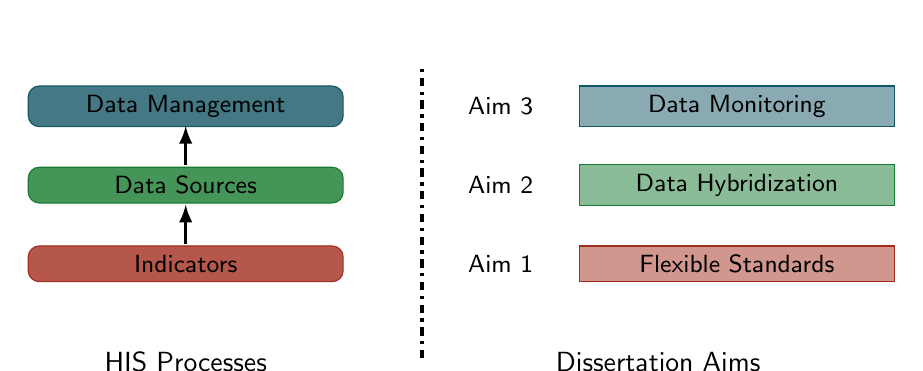
\begin{tikzpicture}

\node[draw , draw = blue ,  fill= blue!80 , minimum width=4cm , rounded corners] at (0,2){\small Data Management} ;
\node[draw , draw = green ,  fill= green!80 , minimum width=4cm , rounded corners] at (0,1) {\small Data Sources} ;
\node[draw , draw = red ,  fill= red!80 , minimum width=4cm , rounded corners] at (0,0) {\small Indicators} ;
\node[below] at (0,-1) {HIS Processes} ;

\draw[very thick , -latex] (0, 0.25) -- +(0,0.5) ;
\draw[very thick , -latex] (0, 1.25) -- +(0,0.5) ;
\draw[very thick , dash dot] (3, -1.2) -- +(0, 3.7) ;


\node[very thick] at (4,2){\small Aim 3} ;
\node[draw , draw = blue ,  fill= blue!50 , minimum width=4cm] at (7,2){\small Data Monitoring} ;
\node[very thick] at (4,1){\small Aim 2} ;
\node[draw , draw = green ,  fill= green!50  , minimum width=4cm] at (7,1){\small Data Hybridization} ;
\node[very thick] at (4,0){\small Aim 1} ;
\node[draw , draw = red ,  fill= red!50 , minimum width=4cm] at (7,0){\small Flexible Standards} ;
\node[below] at (6,-1) {Dissertation Aims} ;

\end{tikzpicture}

%\end{document}

}
\caption{HIS Processes and corresponding dissertation aims}
\label{fig:process_aim}
\end{figure}
\end{center}


\paragraph{Indicators / Flexible Standards} Defining categories and metrics based on which people are going to be counted is an essential piece of the statistical work \citep{desrosieres_politique_1993}. It is an essential step in the simplification involved in the activity of measurement. The field of Global Heath relies on important taxonomies, like the International Classification of Diseases and on Metrics like the Disability Adjusted Life Years, to unify description and measurement of health across the globe, and allow comparison and benchmarking \citep{murray_towards_2007,murray_health_2008}. Meanwhile, at local level, the use of globally defined metrics may have its limits, as it does not allow adaptation to local contexts and situations. The measure of retention of HIV patients in care is an example of this. Understanding the outcome of patients after they enter care is essential to evaluating HIV care systems performance, and efforts have been made to track measure to inform strategic planning and programs evaluation   \citep{the_global_fund_global_2014}. Meanwhile, the measure used in most settings, namely the proportion of patients that are considered \gls{ltfu} after a certain time in care, is an indicator that was originally designed and used in clinical research settings. The high variation of  \gls{ltfu} rates between programs and the low specificity of this metric leads researcher to question the way Loss to Follow Up is defined and retention is measured globally \citep{chi_universal_2011,yehia_comparing_2012,grimsrud_impact_2013,forster_electronic_2008}. Using \gls{emr}, I will model how the measure of retention is affected by local contexts and data quality, and I will explore  more robust ways to measure retention in HIV care.

\paragraph{Data Sources / Data Hybridization} Unavailability of population data in a large number of countries is a well known issue \citep{mahapatra_civil_2007,mikkelsen_global_2015}. As a result, spatial distribution of populations, an essential piece of evidence to develop public health policies, is often unavailable at a policy relevant scale. To palliate these shortcomings, approaches for mapping of populations have been developed, involving the use of macro-level rasters of covariates such as land coverage or night lighting imagery \citep{linard_population_2012,stevens_disaggregating_2015}. These approaches give interesting insights into how populations are distributed, and their output can easily be used for other public health work using the GPS coordinates system. Meanwhile, in situations with very low information on populations, the results of these top-down approaches is often little more than an overlay of covariates. Additionally, their results are hard to use for public health policy planning, as they do not link population to commonly used localization conventions such as places names. My second aim is to hybridize multiple data sources on population to produce a population map of Niger linked to the lowest level of population settlement possible.

\paragraph{Data management / Data Monitoring} Data quality is an important concern of Health Information Systems professionals \citep{shrestha_data_2000} who link it directly to the ability of Information systems to provide good information \citep{mphatswe_improving_2012}. The definition of data quality is directly linked to an idea of trustworthiness, which may affect the use of certain data sources to generate evidence \citep{gimbel_assessment_2011}, and the quality of health data receives a large amount of attention even from high level actors in Global Health \citep{abou-zahr_better_2010}. The best way to ensure data quality is through routine audits of primary data \citep{ronveaux_immunization_2005}. Meanwhile, this approach is costly and may have some cost-efficiency issues. Additionally, it makes little use of historical data, which makes it vulnerable to issues in primary data. My third aim will be to develop a cost effective approach to data quality screening informed by historical data and including a notion of risk attached to data quality.

\subsection{Novelty and scientific contribution}

My dissertation is contributing to three main areas of research surrounding Health Information Systems. One is mostly investigated by the \gls{ict} and interrogates the importance of local adaptation of information systems and its impact on the definition of standards. The second domain of relevance is more linked to the Global Health field, and on works that interrogate how data collected inside health systems can be used to best inform decision making. The last domain of contribution is mainly of interest for the statistical field, and explores the use of statistical methods for surveillance in applied fields.

\subsubsection{Local Adaptation and flexible standards}

In the ICT field, defining standards for data collection systems that can be implemented at local levels but respond to national or international norms. Jørn Braa, describing the approach that presided to the design and development of the \gls{dhis2} remarks that "the top-down and all-inclusive approach to standardization [is] common among ministries and central agencies" and pleads for \textit{flexible standards} following the idea that "the individual standards must be crafted in a manner which allows the whole complex system of standards to be adaptive to the local context" \citep{braa_developing_2007}. The need for local adaptability of Information Systems is seen as a key issue of \gls{ict} in developing countries \citep{macfarlane_harmonizing_2005,walsham_research_2006,walsham_foreword:_2007,jacucci_standardization_2006} and thus some \gls{ict} solutions have been designed and explored in the forms of tools like \gls{dhis2} or standards like the Open Health Information Exchange initiative.

Aims 1 and 3 explore ways in which standards for indicators definition or for the evaluation of data quality can be adapted to specific contexts. In both situations, flexibility is introduced through objective rules : specificity and robustness of the measure of retention in the Aim 1, and cost-effectiveness in the Aim 3. The two rules are different in nature, as one is internal, and based on the characteristics of the data while the other is external, and based on operational characteristics such as the cost of supervision. This approach is innovative, and can be applied to a diversity of questions. An extension of this work could also be the definition of methods for aggregation and comparison of metrics defined and measured using flexible standards.

\subsubsection{Imperfect data Usage}


Health Information Systems data is often underused, or not used at all by its intended users\citep{health_metrics_network_framework_2008}. This underuse is often blamed on the  perceived bad quality of primary data that would make it unfit for statistical analysis
\citep{ronveaux_immunization_2005,makombe_assessing_2008,heunis_accuracy_2011,gimbel_assessment_2011,who_assessment_2011,hahn_where_2013,kihuba_assessing_2014,glele_ahanhanzo_data_2015}. Approaches to solve this issue have mainly focused on improving primary data quality to improve data use  \citep{braa_improving_2012,mutale_improving_2013,ledikwe_improving_2014,nisingizwe_toward_2014}, but some authors have also pointed to the possibility to use even imperfect routine data to answer specific public health questions\citep{gething_improving_2006,gething_information_2007,wagenaar_using_2016}. These approaches rely on the nature of routine data, which is usually highly dimensional and structured times series. This type of data enables the use of robust modeling methods at an adequate level of aggregation, to control and correct for data errors.

My dissertation contributes to this line of research in two different ways.

Aim 1 and 3 also offer improved insights in routine data quality and its impact on health indicators. Aim 1  explores a micro level modeling of data quality and its impact on the measure of patient retention. It will also define retention indicators less sensitive to data quality. Aim 3 uses expected value imputation and aberrant values detection, which is an essential aspect of understanding data quality. It will also implement solutions  to analyze and present the type of data often observed in health systems.

Aim 1 and aim 2 also examine methods to enrich data, using \gls{emr} metadata or  hybridizing different data sources. Both approaches are an extension of usual approaches to health data, and make full use of the richness of modern data collection tools, and of the wide availability of public data sources.

\subsubsection{Statistical methods for health data monitoring}

For aim 3, I am interested in three types of literature that address issues of health data monitoring:
epidemiological surveillance, health service quality monitoring and industrial \gls{spc}.

I will explore a combination of those approaches to provide actionable information on available data in a health system. Indeed, all of these approach rely on a common method, based on the theoretical definition of an expected distribution of some indicator, and then defining a test to classify the observed values as coming from an \textit{in control} or \textit{out of control} process. Using a rare and important data set, I will test and benchmark different algorithm on their ability to detect different types of \textit{out of control} situations.

In the meantime, my implementation of  quality monitoring algorithms will differ from existing literature in an essential way. In most quality monitoring applications, the quantity of interest is the success of some type of procedure, measured by an outcome, of which death is usually the least desirable. In the context of Results Based Funding, on the other hand, the measure of success is much more a measure of access to a wide range of services. The denominator of such a measure is much less clear, as it is not defined at facility level, and there is often little information on target populations. I will thus use methods recently developed in the \gls{spc} field, which aim at monitoring profiles of indicators sets, in order to detect diverging patterns from a standard situation\citep{woodall_current_2014}.  The use of Profile Monitoring for this project is an important innovation in the field of surveillance.

\subsection{Timeline}

Aims specific timelines are explained in more detail in sections \ref{timeline:aim1}, \ref{timeline:aim2} and \ref{timeline:aim3}. I will prioritize getting early results on Aim 2 to allow feedback and field testing from Bluesquare and have an opportunity to reorient my methods if needed. This will also leave time me to obtain potential additional data for Aims 1 and 3. All the aims should be finalized and papers written by the end of the first quarter of 2018, which would allow for a finalization of the dissertation by June 2018.


\begin{figure}[!ht]
	\begin{ganttchart}[vgrid ,
                    hgrid,
                    y unit chart=.6cm]{1}{18}
		\gantttitle{2017}{12}
		\gantttitle{2018}{6} \\
		\gantttitlelist{1,...,12}{1} \gantttitlelist{1,...,6}{1}\\

        \ganttset{bar/.append style={draw=red!40 , fill=red!40},
                    group/.append style={draw=red, fill=red}}
		\ganttgroup{Aim 1}{1}{16} \\
        \ganttbar{Data Extraction}{1}{4} \\
		\ganttbar{Modeling and Model estimation}{5}{6} \\
		\ganttbar{Cohort Simulation}{7}{9} \\
		\ganttmilestone{Sharing Cohort simulation results}{9} \\
		\ganttbar{Data Quality Impact}{10}{10} \\
		\ganttbar{Data Maturity}{11}{12} \\
		\ganttbar{Robust Measures of retention}{13}{14} \\
		\ganttmilestone{Sharing Final Results}{14} \\
		\ganttbar{Paper Writing}{15}{16} \\
		\ganttmilestone{Paper Submission}{16} \\

        \ganttset{bar/.append style={draw=green!40 , fill=green!40},
                    group/.append style={draw=green, fill=green}}
        \ganttgroup{Aim 2}{1}{16} \\
        \ganttbar{Data Extraction}{1}{3} \\
		\ganttbar{Name Matching}{1}{6} \\
		\ganttbar{Locality Mapping}{7}{9} \\
		\ganttmilestone{First complete map}{9} \\
		\ganttbar{Population Estimation}{10}{14} \\
		\ganttmilestone{Sharing Final Results}{14} \\
		\ganttbar{Paper Writing}{15}{16} \\
		\ganttbar{Dashboard Design}{15}{16} \\
		\ganttmilestone{Paper Submission}{16}\\

        \ganttset{bar/.append style={draw=blue!40 , fill=blue!40},
                    group/.append style={draw=blue, fill=blue}}
        \ganttgroup{Aim 3}{1}{14} \\
        \ganttbar{Data Extraction}{1}{1} \\
		\ganttbar{Data Screening}{2}{7} \\
		\ganttmilestone{Sharing Data Screening results}{7} \\
		\ganttbar{Risk Classification}{8}{9} \\
		\ganttmilestone{Risk classification results}{9} \\
		\ganttbar{Supervision Planning optimization}{10}{11} \\
		\ganttmilestone{Sharing Final Results}{11} \\
		\ganttbar{Paper Writing}{12}{14} \\
		\ganttmilestone{Paper Submission}{14}\\
	\end{ganttchart}
	\caption{Dissertation Timeline}
\end{figure}

\clearpage
\section[Flexible Standards]{Aim 1 - Flexible Standards for categories definition}

The measure of retention of ART patients in treatment is a key measure of HIV programs performance. HIV being a chronic disease, the measure of success of these treatments is indeed the survival of treated, patients, which is directly dependent to their adherence to ART treatment. As HIV programs have been rolled out in different countries, the importance of Lost to Follow Up patients (LTFU) in ART cohorts has been recognized, and since the early days of HIV care programs, efforts have been made to better measure and understand the phenomenon \cite{ioannidis_predictors_1999,lebouche_incidence_2006,moh_incidence_2007}.

Initiating treatment programs, HIV practitioners used the categories that had been developed and used in clinical trials to categorize patients outcome. The definition of LTFU used in HIV programs thus comes from settings with highly controlled data collection and close patients follow-up. This definition is nonetheless problematic for public health treatment settings, as it is mainly a negative category, grouping patients who failed to attend their medical appointments and for which no definitive had been recorded. LTFU is thus defined by an absence of data about a patient more than by a positive element of information.

As HIV programs were rolled out, it soon became clear that the LTFU category, in many settings, is a mixed bag of patients with different status \cite{kwong-leung_yu_true_2007,dalal_characteristics_2008,mcguire_vital_2010}. This poses problems for HIV programs evaluation, as the true outcome of HIV patient is often unknown, and different authors have proposed ways to correct retention measures by collecting additional data \cite{yiannoutsos_sampling-based_2008,geng_tracking_2010,tassie_evaluation_2010}, or by fitting correcting models \cite{brinkhof_adjusting_2010,egger_correcting_2011,van_cutsem_correcting_2011,henriques_comparison_2012,verguet_incorporating_2013}.
Finally, some authors started paying attention to how the very definition of patients retention could heavily impact the evaluation of HIV programs performance \cite{chi_empirical_2010,chi_universal_2011,fox_defining_2012,mugavero_measuring_2012,yehia_comparing_2012,grimsrud_impact_2013,shepherd_impact_2013}.

An important underlying hypothesis of retention definition is that, if the patient had been coming to the facility for an appointment, this visit would have been recorded. This hypothesis makes sense considering the notion of LTFU comes from the clinical trial setting\cite{lebouche_incidence_2006}. There is thus an equivalence established between patient's status and data quality in the facility. Meanwhile, assessing data quality of a database and its impact on the measure of retention is very difficult and seldom made. As a result, most reports on LTFU report high variations of results, and unsatisfactory sensitivity of LTFU rates on retention definition. %% Citer Lurton

With the development and rollout of Electronic Medical Records (EMR) in facilities, there is an opportunity to improve on this situation. Most computerized data collection systems collect metadata on data entry, such as the date at which a form was entered, or the role of the person doing the data entry. This metadata could be mobilized to measure the quality of the data, and to understand the impact of data quality on the measure of retention.

This project main aim is to simulate and describe the impact of data quality on the measure of retention of patients in HIV cohorts. This will be achieved using three specific aims :

\begin{description}
	\item[Impact of data quality on the measure of retention] We will model the path through which data quality impacts the measure of retention, and will simulate the results of an HIV cohort with varying data quality.
	\item[Data Maturity] As the time to data entry is an essential element of data quality and directly impacts the measure of retention, the ability to properly measure retention for a given periods improves in time. We will define a metric of data maturity to describe the ability of a database to properly measure retention for a cohort. This measure will be tested and validated on a simulated cohort.
	\item[Robust Retention Metrics] Building on the insight gained in our previous aims, we will define, test and validate different robust retention metrics for HIV cohorts. These metrics will be evaluated on their ability to properly measure the retention of patients in a simulated cohort, and on their robustness to varying data quality.
\end{description}


\subsection{Data Generation Process}

\subsubsection{HIV care process}

HIV patients are visiting hospitals for regular appointments. At each visit, they are given an appointment for their next visit. The date for the $v^{th}$ visit of patient $i$ is noted $V_v^i$, and the appointment time for this visit is noted $A_v^i$. Thus, if $V_v^i > A_v^i$, the patient came late to his appointment, if $V_v^i < A_v^i$, the patient came early. We note $l_v^i = A_v^i - V_v^i$, the lag between scheduled appointment and actual visit. Figure \ref{fig:late_days} shows the distribution of $l_v^i$ in our data. Unrecorded appointments are handled by divided the time between scheduled appointment and actual visit by 28, and consider the remainder. The spikes around 7, 14 and 21 days show either patients who were given an unrecorded appointment of less than a month, or is proof to the fact that patients have favorite days of visit.

\begin{center}
\begin{figure}[ht]
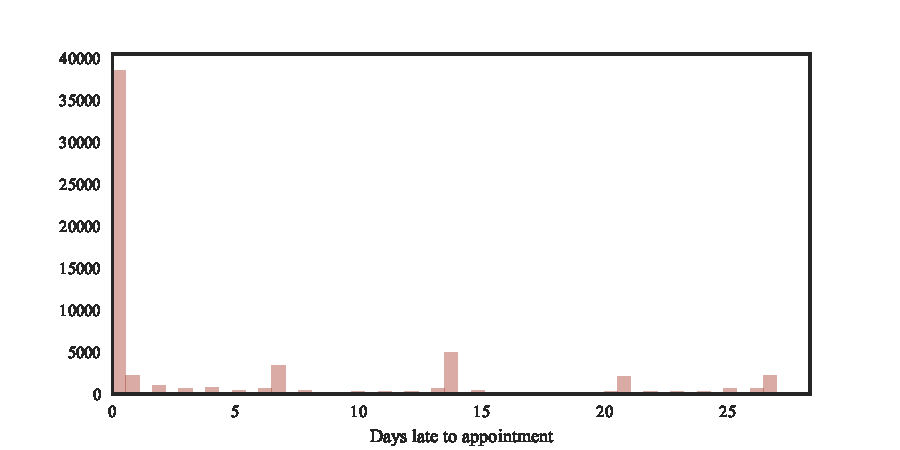
\includegraphics[width=\textwidth]{figure/time_late_to_appointment.pdf}
\caption{Distribution of $l_v^i$ in our data.}
\label{fig:late_days}
\end{figure}
\end{center}

The time between a visit and the next schedule appointment is set by the norms regarding the frequency at which patients should be evaluated, depending on their condition and medical history. Patients recently enrolled in care will be seen more frequently than patients with a longer history and no complications. We note ($\bar{f}_{vi}$) the visit frequency regimen of patient $i$ at visit $v$. This unit is usually around a multiple of 28 days, as patients are likely to have a favorite week day for visit. Figure \ref{fig:schedule_days} shows the distribution of $f_v^i$ in our data.

\begin{center}
\begin{figure}[ht]
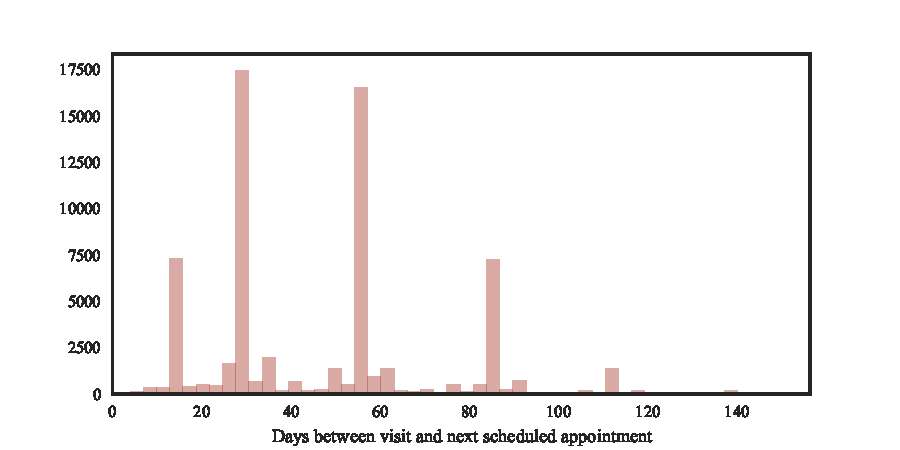
\includegraphics[width=\textwidth]{figure/time_to_appointment.pdf}
\caption{Distribution of $f_v^i$ in our data. We see the visits are scheduled mainly 7, 28, 56 or 84 days after the previous visit}
\label{fig:schedule_days}
\end{figure}
\end{center}

We can finally express the time between two visits as :
$$V_{v+1}^i - V_v^i = \bar{f}_{vt} + l_v^i  $$

\subsubsection{Data Entry}

The date at which a visit is recorded in an EMR database is $R(V_v^i)$. By definition, $R(V_v^i) \geq V_v^i$, and the delay in data entry is noted :
$$R(V_v^i) - V_v^i = \delta_v^i \ geq 0$$

In some cases, the visit has not and will never be recorded, and we will note this situation as $\delta \rightarrow \infty$. $\delta$ may vary in a facility, depending on the workload, staffing or other factors. Figure \ref{fig:data_entry_time} shows the distribution of $\delta$ in our data.

\begin{center}
\begin{figure}[ht]
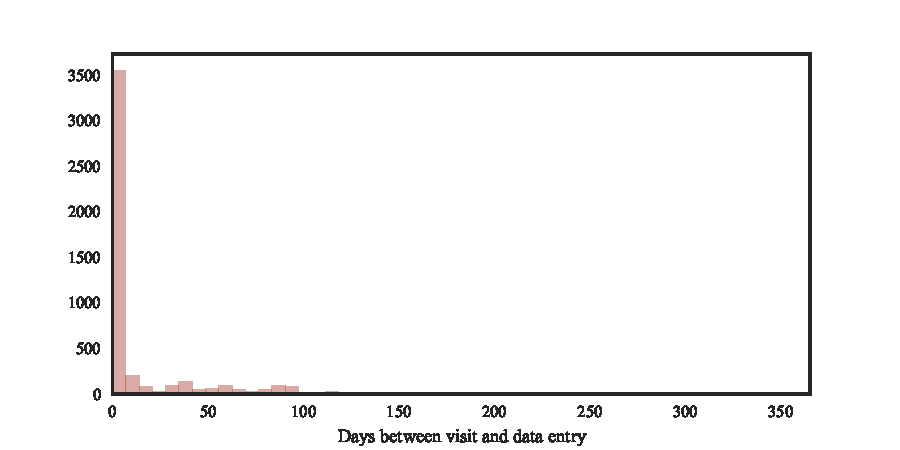
\includegraphics[width=\textwidth]{figure/data_entry_time.pdf}
\caption{Distribution of $\delta_v^i$ in our data. Most of the data is entered in the first week following the visit, but we see some data can be entered much later}
\label{fig:data_entry_time}
\end{figure}
\end{center}

Finally, data entry is interrupted at the date $T_{close}$ before the data is used for analysis. The time elapsed between patient $i$'s last visit and the closing date is noted as $G_i = T_{close} - \max_v(A_v^i)$. For simplicity, we will equate the date of database closure with the date of analysis in a first step, and will relax this assumption when we will be measuring data maturity.


\pgfdeclarelayer{background}
\pgfdeclarelayer{foreground}
\pgfsetlayers{background,main,foreground}
\begin{center}
 \begin {figure}[ht]
        \centering
\resizebox{\linewidth} {!} {
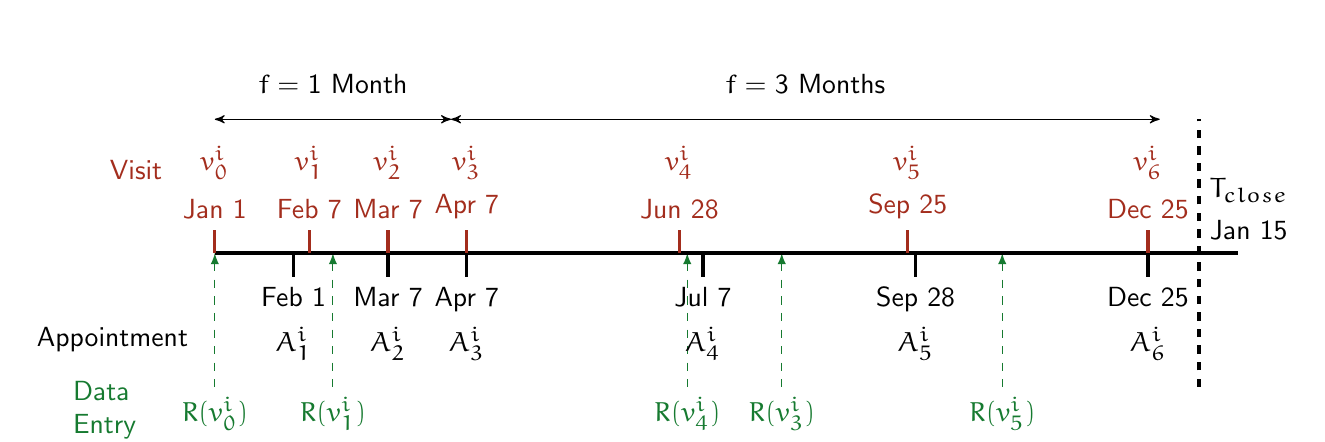
\begin{tikzpicture}


  \draw[<->] (0,1.7) -- (3,1.7);
  \draw[] (1.5,1.9) node[above]{$f =$ 1 Month};
  \draw[<->] (3,1.7) -- (12,1.7);
  \draw[] (7.5,1.9) node[above]{$f =$ 3 Months};


  \draw[ very thick] (0,0) -- (13,0);

\begin{pgfonlayer}{main}
  %% Draw Appointments
  \draw[very thick] (-1.3,-8mm)node[below]{Appointment};
  \foreach \x/\y/\z in {1/Feb 1/$A_1^i$,
                     2.2/Mar 7/$A_2^i$,
                     3.2/Apr 7/$A_3^i$,
                     6.2/Jul 7/$A_4^i$,
                     8.9/Sep 28/$A_5^i$,
                     11.85/Dec 25/$A_6^i$
                     }{
 \draw[very thick] (\x, 0) --+ (0,-3mm) node[below](\x){\fontsize{20}{22.4}\y}(\x,-8mm)node[below]{\z};
 }


  %% Draw Visits
  \draw[red , very thick] (-1,8mm)node[above]{Visit};
  \foreach \x/\y/\z in {0/Jan 1/$v_0^i$ ,
                     	1.2/Feb 7/$v_1^i$,
                     	2.2/Mar 7/$v_2^i$,
                     	3.2/Apr 7/$v_3^i$,
                     	5.9/Jun 28/$v_4^i$,
                     	8.8/Sep 25/$v_5^i$,
						11.85/Dec 25/$v_6^i$
                        }{
	\draw[red , very thick] (\x, 0) --+ (0,3mm) node[above](\x){\fontsize{20}{22.4}\y}(\x,8mm)node[above]{\z};
    }
\end{pgfonlayer}

\begin{pgfonlayer}{background}
    %% Draw Data Entry
    \draw[very thick ,  green] (-1.4,-25mm)node[above , align=left]{Data\\Entry};
    \foreach \x/\y in {0/$R(v_0^i)$,
  					   1.5/$R(v_1^i)$,
					   6/$R(v_4^i)$,
                       7.2/$R(v_3^i)$,
                       10/$R(v_5^i)$
                        }{
    \draw[dashed ,  green , latex-] (\x,0mm) -- +(0,-17mm)node[below]{\y};
    }

\draw[dashed ,  very thick] (12.5,-17mm) -- (12.5,17mm) ;
\draw[very thick] (12.5, 8mm)node[right]{$T_{close}$};
\draw[very thick] (12.5, 3mm)node[right]{Jan 15};

\end{pgfonlayer}

\end{tikzpicture}

}
\caption{Individual follow-up and data entry process}
\label{fig:timeline-followup}
\end{figure}
\end{center}

Figure \ref{fig:timeline-followup} shows how these different parameters can play out for a given patient. This imaginary patient had a first visit on January 1st, and had an appointment scheduled on February 1st, to which he came 6 days late. After three months of being seen monthly, he switched to a quarterly follow up. He was early to his July appointment, but came to every appointment until the end of the year. The data was entered very quick at the beginning of the year, but $v_2^i$ was never recorded. $v_4^i$ was entered before $v_3^i$, and $v_6^i$ could not be entered before the database was freezed for analysis on January 15 of the following year. This example gives a rough demonstration of the different situations and problems that can be encountered when analyzing the follow-up of the patient.

\subsubsection{Loss to Follow Up definition}

A central piece of the LTFU definition is the  \textit{grace period} during which a patient, even if he did not return to a facility, is considered actively followed. This \textit{grace period} is denoted $G_0$.

A patient $i$ is considered actively followed if he is not late to his latest appointment for more than $G_0$ days.

$$l_{v^{*}i} \leq  G_0$$

Looking closer at this definition, we can see it regroups three different situations :
\begin{enumerate}
\item The patient is LTFU and will never come back to the facility
\item The patient is late to his appointment but will come back, and $l_{v^{*},i} > G_0$
\item The patient came for his visit $v^{*} + 1$ but $\delta_{v^*+1} > G_0$.
\end{enumerate}

Using this definition, we can express the probability that patient is identified as LTFU based on the data at hand. Let's $X = 1$ be the event that a patient is actively in care, and $X = 0$ if the patient is LTFU. We can thus get $p(X = 0 | l_{v^{*}i} \leq  G_0)$ as the combination of elements we can measure :

$$p(X = 0 | l_{v^{*}i} \leq  G_0) = 1 - p(X = 1  \cap l_{v^{*}i} \leq  G_0) - p(\delta_{v^*+1} > G_0) $$

We can understand $X = 1  \cap l_{v^{*}i} \leq  G_0$ as the data quality term, and $\delta_{v^*+1} > G_0$ as an intrinsic myopia of the information system on the future. Meanwhile, differentiating between these two terms is  important in order to understand uncertainty in the LTFU rate and better measure retention in the cohort.

\subsection{Data}

The data used for this paper is a Electronic Medical Records database obtained from the HIV program in Kenya during the ABCE study in IHME. In this facility, 4833 patients have been registered for HIV care, from 2005 to June 2012, totaling 69591 recorded visits. Data entry time is easily available for at least 4853 of these visits.

I hope to obtain additional EMR databases from different HIV program. This would allow me to better measure variability in appointments lags and data entry issues. All the data will be analyzed anonymously and in aggregate form. For each patient, I only use visit dates and scheduled appointment dates are used. If schedule appointment dates are missing, they will be imputed using observed visit patterns in the data. I will also use the metadata collected in the EMR, especially the dates of data saving will be used to estimate data quality.

We will not report precise data on HIV programs performance, and all the data used will used to inform our simulation model.

\subsection{Methods}

Our work will be done in three main steps. First, we will estimate the relevant quantities in our model from our data. In a second step, we will simulate a cohort and its monitoring, using estimated quantities as parameters. Finally, we will use this simulation, varying different parameters, to answer our main questions of interest.

\paragraph{Modeling -} The different parameters described earlier will be modeled and estimated  from the cohort data we will have at hand, using a Bayesian approach. The two most important parameters for our work are $\delta$, the time before visit has been recorded in a database, and $l$, the time between an appointment and the actual visit.

$\delta_{v,i}$ can be modeled as a Gamma distribution $\mathrm{G}(\alpha , \beta)$, with mean $\frac{\alpha}{\beta}$ representing the mean time to data entry of a visit form in the EMR. A Gamma distribution allows for a very long tail on the right, which will allow us to include data loss ($\delta  \rightarrow  \infty$)

$l_{v,i}$ will have to be estimated using a mixture model, to take into account the multimodal nature of the $l$. We will also have to consider the hypothesis that the the multimodal lateness distribution results from unrecorded shorter term appointments, and if this is the case we may need to use a long tailed distribution as for $\delta_{v,i}$.

\paragraph{Simulation - } Using the parameters estimated in the previous step, we will simulate an HIV patients cohort. This simulation will be made using the Cost Effectiveness Analysis Microsimulation (CEAM) framework developed at IHME to simulate epidemiological cohorts.

In a second step, we will simulate the data entry process, for any given month, by drawing a $\delta$ for any  visit that has been generated (initial or returning), and then computing the date of data entry for the information related to this visit.

As a result of this simulation, we will have all the information needed to estimate retention and measure of retention for the cohort. Varying selected parameters, we will be able to measure the quantities of interest for our study aims.


\paragraph{Quantities of interest -} This simulated data will then be used to estimate our elements of interest :

\begin{enumerate}

\item{Measuring data quality impact} We can simulate $ p(X = 0 | \theta_{\delta})$ based on different values of the parameters of $\theta_{\delta}$. Different scenarios will be considered for data quality, varying both the mean and variance of $\delta$. Perfect data quality will be compared to situations with long delays of data entry, and situations with important data loss (high variance of $l$). The resulting variation in $p$ will be described as the impact of data quality on the measure of retention.

\item{Data maturity} As data is being entered in the EMR, or as missed visits are being made again, the data for a given period will get completed, and patients actively on care are more and more considered so. As data maturity grows in the EMR, the data quality induced error is lowered. Varying $T_close$ can thus have an impact on the measure of retention of a patient on a given date. We will carry out the measure of retention using different closing dates for the database, and only using the data recorded before the closing date. These measures will allow us to define and test a Data Maturity metric, based on a combination of $\bar{f}$, $l$ and $\delta$ that will allow us to identify the optimal minimum date of analysis to estimate retention rates in a program, and the optimal grace period $G_0$ to use for different levels of maturity.

\item{Robust measures of retention} Finally, we will consider more robust metrics that can be considered good proxies for retention. These metrics will include :
\begin{itemize}
	\item The ratio of the corrected average number of registered visits on the expected number of followed patients
	\item The ratio of new to returning patients in the facility
	\item The probability that the rate of LTFU is higher than a given threshold
\end{itemize}
\end{enumerate}

For each of these metrics, we will evaluate their capacity to measure retention in the cohort, by comparing with the reference measure of LTFU measured with perfect data. We will also evaluate the sensibility of these metrics to data quality and data maturity.

\subsubsection{Timeline}
\label{timeline:aim1}

I am still hoping to obtain additional data for this aim. I anticipate starting to work on the estimation of the model parameters from this data in April 2017. Based on these parameters, I will be able to implement the cohort and data entry simulation and will have first results to share on this simulation in September 2017. Based on this simulation, I will estimate data quality impact, data maturity impact and I will test robust measures of retention during the last quarter of 2017 and the first quarter of 2018, and I plan on having final results by February 2018. Figure \ref{GanttPaper1} summaries this timeline.

\begin{figure}[!t]
	\begin{ganttchart}[vgrid,hgrid,
	y unit chart=.6cm]{1}{18}
		\gantttitle{2017}{12}
		\gantttitle{2018}{6} \\
		\gantttitlelist{1,...,12}{1} \gantttitlelist{1,...,6}{1}\\

		\ganttset{bar/.append style={draw=red!40 , fill=red!40},
					group/.append style={draw=red, fill=red}}
		\ganttbar{Data Extraction}{1}{4} \\
		\ganttbar{Modeling and Model estimation}{5}{6} \\
		\ganttbar{Cohort Simulation}{7}{9} \\
		\ganttmilestone{Sharing Cohort simulation results}{9} \\
		\ganttbar{Data Quality Impact}{10}{10} \\
		\ganttbar{Data Maturity}{11}{12} \\
		\ganttbar{Robust Measures of retention}{13}{14} \\
		\ganttmilestone{Sharing Final Results}{14} \\
		\ganttbar{Paper Writing}{15}{16} \\
		\ganttmilestone{Paper Submission}{16}
	\end{ganttchart}
	\caption{Gantt Chart for Aim 1}
	\label{GanttPaper1}
\end{figure}

\clearpage
\section[Data hybridization]{Aim 2 - Data hybridization for population mapping in Niger}

In 1935, British geographer Charles Fawcett defined three phenomenons that could be described on a population map \citep{fawcett_population_1935}:
\begin{enumerate}
	\item The actual number of the people within given areas
	\item The density of the population in these areas
	\item The grouping, or arrangement, of the population in space.
\end{enumerate}

Each of these elements is important to design public health programs, to plan infrastructure development or to implement quick emergency response \citep{bambas_nolen_strengthening_2005,thieren_health_2005}. Meanwhile, the lack of good quality data on populations size and locations in low resource and developing countries is well known \citep{mikkelsen_global_2015}. As a consequence, most current approaches to population mapping rely on models  aimed at mapping density surfaces \citep{linard_population_2012}. This approach makes best use of the availability of large datasets for land use and other usable covariates, and of the computational ability to interpolate these  different data sources for population distribution\citep{stevens_disaggregating_2015}. As is evident for Niger in Figure \ref{AfriPopMap}, in countries with little urbanization, and poor population data, these methods end up displaying an overlay of covariate layers more than they present a credible distribution of populations.

\begin{figure}
	\begin{center}
	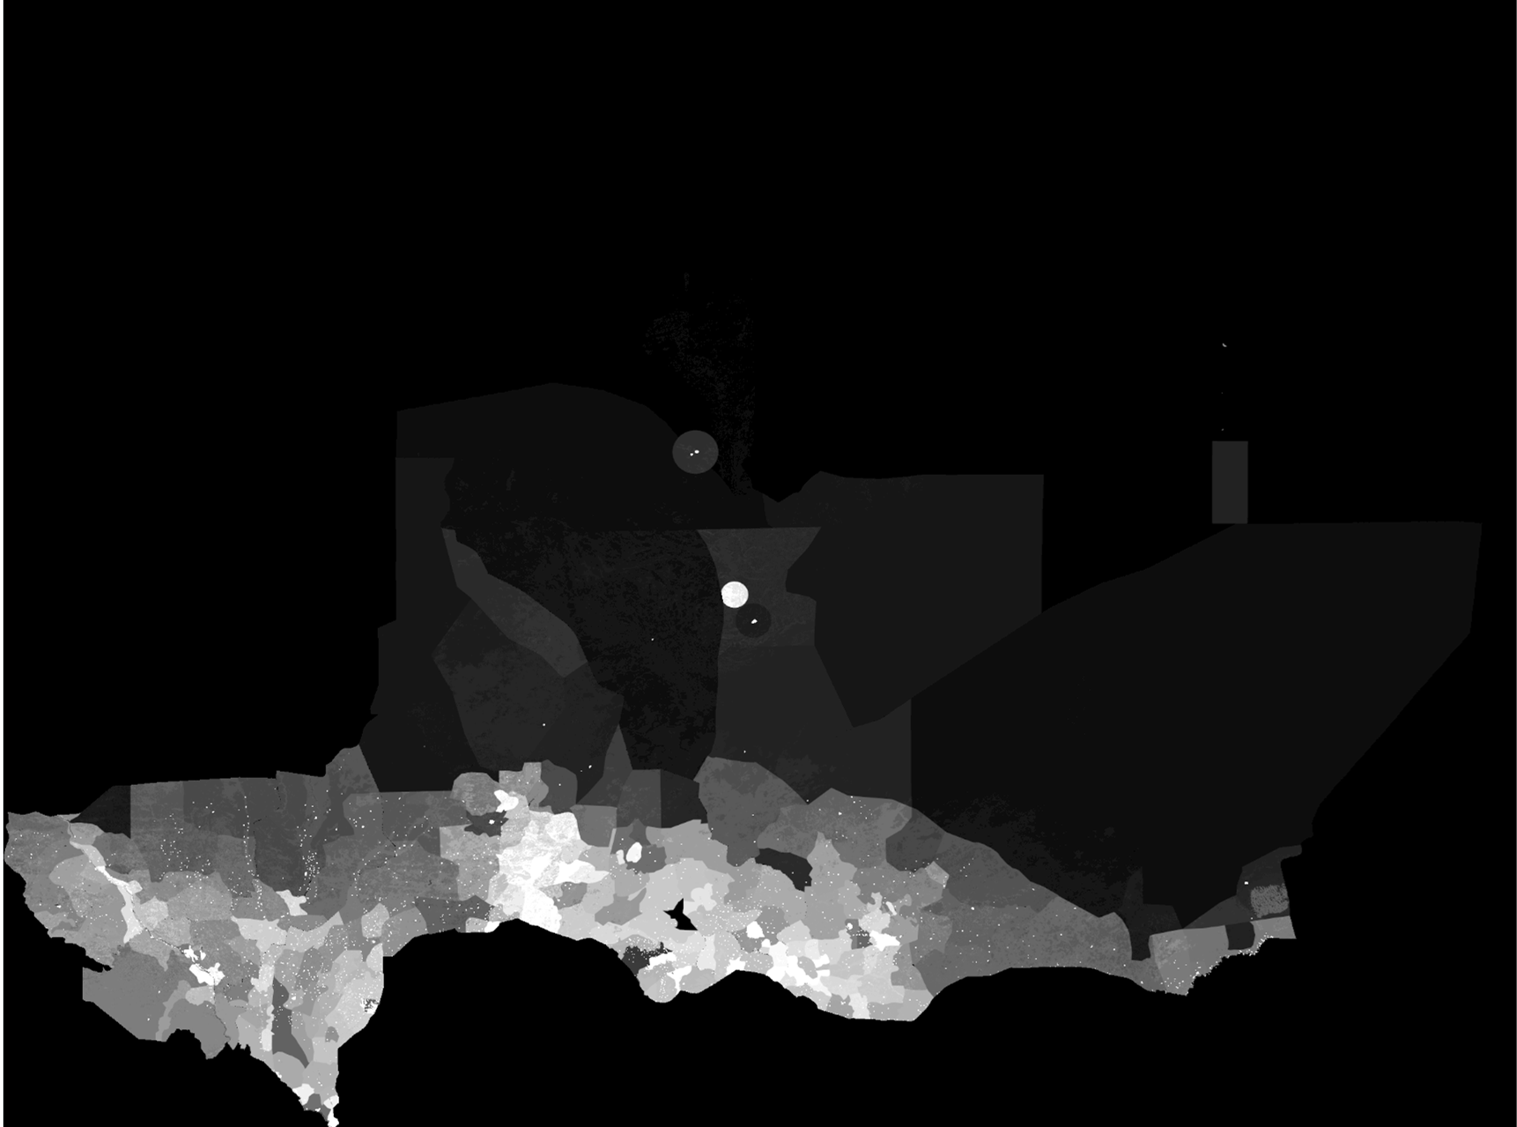
\includegraphics[width=0.8\textwidth]{figure/WORLDPOP_Niger.png}
	\caption{Mapping of Niger population from AFRIPOP}
	\label{AfriPopMap}
	\end{center}
\end{figure}

Mapping the density of the population is useful for descriptive purposes, and the production of density rasters can be essential to the spatial modeling of diseases and other population phenomenons. Meanwhile, these maps do not display actual numbers of people, nor a comprehensive display of populations groupings. Moreover, being able to query places by their name is an essential feature for managers. The information needed to produce a precise and actionable map of population in Niger can be found scattered in different unrelated data sources. This  project is exploring an innovative approach to provide a population map in Niger, through the hybridization of multiple data sources and the use of Bayesian models for administrative data.

\subsection{Data}
\lable{aim2:data}

\paragraph{Voters list as a demographic data source} A data source that is, to my knowledge, seldom used to inform population mapping for public health purposes, is voters registration lists. This low usage can be linked to concerns regarding the completeness of this data in settings where only subsets of the population are eligible to vote, to issues regarding the regular update of this lists, or to the political purported use of these data, that could favor non-random missingness in data in some situations.

There is meanwhile a case to be made for the use of voters' registration data to estimate size and the spatial distribution of populations. By definition, voters' registration should aim at being as complete as possible a register of adults in the nation. Moreover, in most democracies, some form of national elections are held at least  every five years, leading to an update at least partial of voters' registrations. In sub-Saharan Africa, between the years 2015 and 2016, 27 countries were supposed to hold national elections, leading to a theoretical registration of more than half of the adult population of the continent. Finally, for transparency and accountability reasons, electors registries are supposed to be accessible.

Due to the sensitive and political use of these data, the quality of voters registries are often described as not being trustworthy. On the other hand, for the same sensitivity reasons, voters registries are receiving a high level of scrutiny from different actors, and are audited sometimes multiple times before validation. This level of scrutiny before validation is much higher than the attention given to a lot of studies or other often used data sources.

\paragraph{The Niger 2016 elections voters registry} In Niger, presidential and parliamentary elections were held in February 2016. Voters lists were updated during the second half of the year 2015, under the supervision and control of a mission of the \gls{oif}. The operations for registration of voters were conducted during the third quarter of 2015\footnote{\url{http://www.ceni-niger.org/article-region/##more-24}}.
A first version of the voters list was published on December 21, 2015, tallying 7,569,172 voters, out of 8,569,309 that were expected based on the 2012 census\footnote{\url{http://www.iinanews.org/page/public/news_details.aspx?id=98929&NL=True}}

Final lists were validated in early January 2016 after being corrected for some incoherencies noted by the supervisory body\footnote{\url{http://www.nigerinter.com/2016/01/le-fichier-electoral-du-niger-valable-sous-reserves/}}.
A final report on these lists was published in may 2016\footnote{\url{http://www.nigerinter.com/2016/05/remise-officielle-du-rapport-du-fichier-electoral-au-ministre-detat-a-linterieur-par-le-cfeb/}}.
The \gls{ceni} later made these lists fully available on its website, from which I extracted, anonymized and formatted the lists.

\paragraph{RENALOC and RENACOM} The \gls{renaloc} is a geolocalized repertory of all localities in Niger.  The 2012 version was downloaded as a pdf file from the \gls{ins} website. The tables were extracted in bulk from this file using the Tabula Package, and then processed in Python to recompose the geographic structure of the document. The final data consists in 34507 localities, for which the INS provides the number of inhabitants, by gender, as well as the number of households, and the number of agricultural households. For most of the localities, a GPS coordinate is recorded, as well as the type of locality (neighborhood, village, camp, water well, hamlet).

The 2001 version of this database, named \gls{renacom}, contains similar information. Meanwhile, the number of places identified varies, and for places identified in \gls{renaloc} and \gls{renacom}, some names spelling vary. I retrieved the \gls{renacom} in Excel tabular format directly from the \gls{ins} website.

\paragraph{OpenStreetMap} \gls{osm} is "a free, editable map of the whole world that is being built by volunteers largely from scratch and released with an open-content license"\footnote{\url{http://wiki.openstreetmap.org/wiki/About_OpenStreetMap}}. Its API allows an easy query of its content, from which we can retrieve places names and community generated GPS coordinates. This data can provide additional precisions on where some localities are, but is much less complete than both \gls{renaloc} and \gls{renacom}.

\paragraph{DHI2} The Niger \gls{snis} is currently implementing \gls{dhis2}. The portal to \gls{dhis2} already makes available some limited geolocalization data, regarding the health districts divisions, and some health facilities coordinates\footnote{\url{http://www.snisniger.ne/dhis-web-commons/security/login.action}}.


\subsection{Methods}

To make the best use of this data, I will implement an approach based on a minimal modelling of primary population data, and geared towards the anchoring of population in callable named localization. To achieve this, my project has three main components.

\subsubsection{Name Matching}

Due to the history of the creation and administration of the Nigerien territory, multiple different spellings are in use for most localities names in Niger. There are no obvious reasons to prioritize one spelling over another for this project. To the contrary, I want users to be able to use whichever spelling of a name they prefer to query their results.

In collaboration with Fahad Pervaiz, a PhD student in the department of Computer Science at UW, I am designing a matching algorithm for different spellings of the same locality names in Niger. Our approach relies on the use of  a mixture of standard string matching algorithms. We use these algorithms for each pair of data sources and define a heuristic to combine them and select best matches. We also enrich these heuristics by defining patterns and features that allow a first classification and simplification of names to improve matching performance. These patterns may be data source specific to reflect explicit or non-explicit conventions used in each data source.

After this first round of unsupervised matching, we will manually confirm some of the matches with the help of members of the \gls{osm} community in Niger. Using this validated training set, we will fit supervised algorithms to improve our previous matching approach.

As a result of this step, I will have a consolidated list of localities in Niger, with different possible spellings of names for each of them.

\subsubsection{Locality mapping}

The three data sources that include GPS coordinates (\gls{renaloc}, \gls{renacom}, \gls{osm}) have GPS coordinates for different subsets of localities in Niger. It appears that \gls{renaloc} GPS coordinates are of very low quality, and that \gls{osm} coordinates are sometimes rough estimates of exact locations with a rounding factor. I will design an algorithm to attach, for each identified locality, the most probable GPS localization.

\begin{enumerate}
\item Get \gls{renacom} GPS coordinates for localities where they are available.
\item Fit some models to correct GPS coordinates in gls{renaloc} using localities with both \gls{renaloc} and \gls{renacom} GPS coordinates. Use the best performing approach, as evaluated with cross-validation, to correct RENALOC coordinates
\item Fit some models to correct GPS coordinates in \gls{osm} using localities with both \gls{osm} and \gls{renacom} GPS coordinates. Use the best performing approach, as evaluated with cross-validation, to correct \gls{osm} coordinates
\end{enumerate}

For steps 2 and 3, different linear models will be tested, as well as non linear Machine Learning approaches allowing for different local corrections. For localities with \gls{renaloc} and \gls{osm} coordinates but no \gls{renacom}, I will evaluate if the results 2 or 3 or a combination of both performs best, using localities with GPS from the three data sources as training set.

As a result of this step, I will have the most complete and accurate grid possible of named localities in Niger.

\subsubsection{Population modeling}

Finally, I will model Niger population using its voters list by voting precinct as a main data source. I could not source an example of using voters list as a source for demographic estimation. Meanwhile, in a country like Niger where elections are held much more regularly than censuses, using voting lists, a quasi complete enumeration of the population, to estimate population size and structure, does not seem unreasonable.

\begin{figure}[ht]
	\begin{center}
		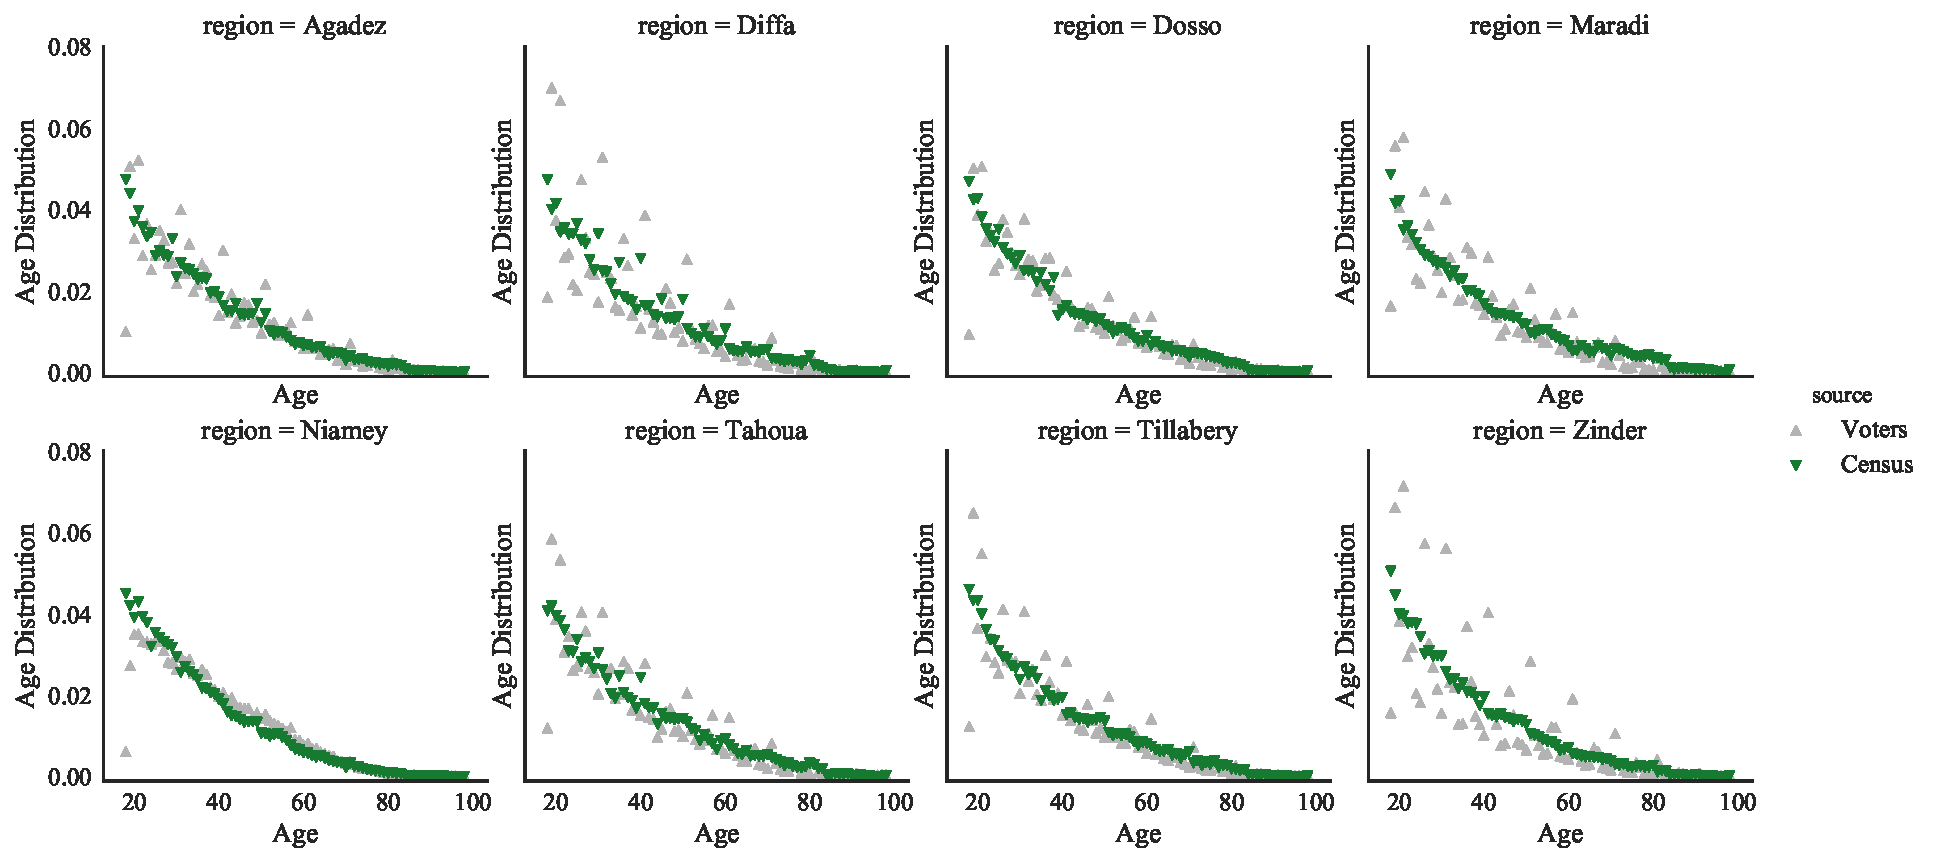
\includegraphics[width=\textwidth]{figure/age_structure_comparison.pdf}
		\caption{Comparison of standardized adult age distribution between the 2012 census and the 2016 voting lists}
		\label{fig:age_comparison}
	\end{center}
\end{figure}

A specificity of the voting list is that it does not include children under 18, as they are not allowed to vote. Additionally, I listed in section \ref{aim2:data} some issues that can be raised regarding the quality and completeness of voters lists, and I should assess their quality and correct their count to match the census results. Finally, as voting lists are very local, I will need to determine the most appropriate level of aggregation to get a meaningful estimation of the population age and gender distribution. Figure \ref{fig:age_comparison} compares the standardized age distribution of adults in the 2012 census and in the 2016 voters list at regional level. We can see there is more variability in the voters lists age structure than in the census. Concordance between the two age distributions seems to vary between regions.

I will model population size and age and gender distribution at regional and health zone level, using the electoral lists as input data, and the 2012 census regional distributions of population by age and gender as validation data. A simple approach will be used to keep this part of the project tractable, and easily reproducible locally. Age distributions from the voters lists will be aggregated at the regional or health zone level, and a number of children will be computed using widely available life tables. I will use multiple life tables to get an estimation of uncertainty on this estimation. The total population numbers will then be modeled in a linear regression framework, using the 2012 census numbers as validated results.

\subsection{Output}

The output of the project will  be an interactive map, allowing the query of our results for local practitioners. This dashboard will have the following feature :
\begin{enumerate}
	\item An interactive map of Niger localities, selectable by clicking, or panning for multiple selection
	\item An estimation of the population in the zone selected on the map
	\item A histogram representing the age structure of the population in the localities selected on the map
	\item A search box through which the user will be able to search for a given locality with different spellings. Every name linked to a mapped locality will be searchable and will return the different matching localities in a hierarchized way.
\end{enumerate}



\subsection{Timeline}
\label{timeline:aim2}
I am currently trying to obtain more detailed census data from Niger Census. Meanwhile, the name matching and locality mapping work is already well advanced as we have a first set of matched names from the unsupervised approach, and I have already explored approaches to GPS correction for \gls{renaloc}. I anticipate three more months on the name matching and one month to confirm the locality mapping and the overlay with other \textit{adhoc} layers such as health services and health administration map, and should have completed mapping data by September 2017. I plan 5 months of work for the population estimation, and should have my final results by February 2018. Figure \ref{GanttPaper3} summaries this timeline.

\begin{figure}[t]
	\begin{ganttchart}[vgrid,hgrid,
	y unit chart=.6cm]{1}{18}
		\gantttitle{2017}{12}
		\gantttitle{2018}{6} \\
		\gantttitlelist{1,...,12}{1} \gantttitlelist{1,...,6}{1}\\

		\ganttset{bar/.append style={draw=green!40 , fill=green!40},
                    group/.append style={draw=green, fill=green}}
		\ganttbar{Data Extraction}{1}{3} \\
		\ganttbar{Name Matching}{1}{6} \\
		\ganttbar{Locality Mapping}{7}{9} \\
		\ganttmilestone{First complete map}{9} \\
		\ganttbar{Population Estimation}{10}{14} \\
		\ganttmilestone{Sharing Final Results}{14} \\
		\ganttbar{Paper Writing}{15}{16} \\
		\ganttbar{Dashboard Design}{15}{16} \\
		\ganttmilestone{Paper Submission}{16}
	\end{ganttchart}
	\caption{Gantt Chart for Aim 3}
	\label{GanttPaper3}
\end{figure}

\clearpage
\section[Understanding Information]{Aim 3 - Understanding information - what a bottom up appraoch is}

\subsection{Objective}

As a field, Global Health has to navigate between different levels of relevance. A Global Level, that aims at understanding global trends and phenomenons, and a local level, in which policies are implemented. In this regard, one of the challenges of Global Health is to create and disseminate information that will be relevant at these different levels. The difficulty in doing this is not merely a technical one, but also a political and structural one. The field in which this information is produced is indeed pre-organized by historic and political structures, that are not adapted for this multi-level adaptation of knowledge. National Statistical systems, for example, are the products of the larger systems they are designed to serve. As such, Health Information Systems are the results of the Health Systems in which they are created, and are influenced by the administrative cultures and the political context they are supposed to inform \citep{bergeron_savoirs_2014}.

This relation between local and global levels of Global Health is nonetheless asymmetric. As a scientific field, Global Health is essentially a hierarchical organization, where political, academic and economic institutions situated in high resource countries world offer guidance and validation for the methods and results used to measure health over the world. As a result, the field has to find an equilibrium between a downwards  \textit{standardization} of information and an upward \textit{aggregation} of locally produced data.

The social background in which this equilibrium is sought is important and has its roots in the origins of health information system in developing countries. Whereas European statistical systems development was led by social activists who guided the design of the first modern welfare systems \citep{desrosieres_politique_1993,desrosieres_administrator_1997}, colonial statistical systems were geared towards efficient land administration and economic exploitation \citep{rambert_cartographie_1922,de_martonne_cartographie_1931} with little attention to local population. The development of these statistical systems can indeed be traced to the enforcement of a specific mode of administrative control by colonial powers in the XIXth century \citep{appadurai_number_1996,cordell_couting_2010,gervais_how_2010}.
Colonial statisticians, often weakly skilled or trained \citep{kateb_gestion_1998,cordell_couting_2010}, nonetheless set the nomenclatures and conventions around how land and populations would be described and analyzed \citep{rambert_cartographie_1922,gervais_how_2010}. Enumeration and its categories did not emerge to describe local complexities and specifities, but were on the contrary simplifications aimed at creating a uniform colonial subject, to which a standard colonial rule would apply \citep{said_orientalism_1979,appadurai_number_1996}.


This historical background can be prolonged after the decolonizations, and can present some continuities with the way public health statistics are produced in developing countries today. Understanding how this longstanding history affects the way people involved in Global Health Metrics think about the production of quantitative evidence is important for practitioners of Global Health Metrics to understand the limits of their work, and the improvements they can bring.
% In these settings, strong public health information systems are the result of local equilibria and of adaptations to local statistical cultures, started by individuals making ad-hoc use of different data sources and inventing and standardizing methods on the run. \citep{lecuyer_medecins_1987}.

The aim of this paper will be to provide a clear understanding on how the structure of the field of Global Health can have an influence on how health metrics are produced, and how they are being used, or not used. Providing this framework on the conditions for designing quantitative evidence in Global Health is essential to design useful methods and metrics that can help shape public health policies at local and global levels. I will then use this framework to show how it can help understand and bring into context the results of my applied work.

%The emergence of Global Health Metrics as a field is aimed at providing "valid, reliable and comparable measures of the health states of individuals and of the health status of populations" \citep{mathers_population_2003} This triad of characteristics may be hard to ensure in a single scope, especially when the locally relevant may not be globally comparable. Meanwhile, this paper will explore the hypothesis that the emphasis given to comparability in this triade is historically, intellectually and politically situated, and can be linked to a culture of top-down standardization of knowledge in the developing world.


\subsection{Method}

This paper will build on the work and results of the two previous aims as well as on other work I have done in the field, to understand the conditions in which a \textsl{bottom-up} approach to health metrics can be defined and put into practice. The methodological challenge of this to work is to enter the domain of critique from within my own field \citep{latour_why_2004}. Most of the critical work on the use of quantitative evidence in health policy indeed comes from researchers that are not practitioners of Global Health Metrics \citep{merry_measuring_2011} . In this regard, even the most nuanced critique suffers the temptation of an overwhelming challenge to the possibility of quantitative work\citep{latour_why_2004}.

I will thus offer a framework and examples for an internal critique of this work. Using the opposition between a downward, normative movement and an upward, aggregative movement of methods and data, I will offer a simple explanation of how power relations that structure Global Health Metrics can be found in the methods that are used, and I will show how understanding the limits of these methods can help challenge this power structure, to reequilibrate the relationship between local and global actors of Global Health.

This work will be built in three main parts:

\begin{enumerate}
\item Provide a description of how a top-down approach to Health Metrics differs from a bottom-up approach.
\item Delineate how the structures in place in Global Health can influence which of these approach will be used by Global Health actors.
\item Describe the comparative benefits and shortcomings of each approach, and how they can be combined.
\end{enumerate}

The main methodological challenge of this paper is to make a common reading of literature from \gls{sts}, Colonial Studies and Global Health Metrics. This diverse corpus will be used to test the hypothesis made in other projects in this dissertation, as well as other projects I am involved in. I organize this project in four steps:

\begin{enumerate}
\item Explore the literature in \gls{sts} and Colonial Studies pertinent to the opposition \textit{bottom-up} vs \textit{top-down} of statistical methods.
\item Identify the themes and concepts relevant to the Health Metrics field in this literature.
\item Identify features relevant to these themes in my applied work, and build a critical framework in which to read this my projects.
\end{enumerate}

\subsection{Timeline}
\label{timeline:aim3}

I have already made most of the literature review for this work. A first paper on this work has been accepted for presentation in a workshop at the Ecole des Hautes Etudes en Sciences Sociales. Another presentation of this work for social scientists interested in Data Science should be held at the UW in december. This will allow me to get feedback and to complete my analytical framework. Most of the remaining work for this aim is to include the results from the two other aims and to situate them in my analytic framework.


\begin{figure}[!t]
	\begin{ganttchart}[vgrid,hgrid,y unit chart=.6cm]{1}{9}
		\gantttitle{2017}{3}
		\gantttitle{2018}{6} \\
		\gantttitlelist{10,...,12}{1} \gantttitlelist{1,...,6}{1}\\

		\ganttset{bar/.append style={draw=blue!40 , fill=blue!40},
					group/.append style={draw=blue, fill=blue}}
		\ganttbar{Finalize Litterature review}{1}{4} \\
		\ganttbar{Finalize analytical Framework}{1}{6} \\
		\ganttmilestone{Seminar Presentation}{3} \\
		\ganttbar{Paper finalization}{4}{8} \\
	\end{ganttchart}
	\caption{Gantt Chart for Aim 3}
	\label{GanttPaper3}
\end{figure}

\clearpage


%%%%%%%%%%%%%%%%%%%%%%%%%%%%%%%%%%%%%%%%%%%%%%%%%%%
%% 			BIBLIOGRAPHY
%%%%%%%%%%%%%%%%%%%%%%%%%%%%%%%%%%%%%%%%%%%%%%%%%%%
%\cleardoublepage
\newpage
\phantomsection\addcontentsline{toc}{section}{References}
\bibliographystyle{agsm}
\bibliography{ma_bibliotheque}


\end{document}
